\documentclass[a5paper, 10pt]{article}

% Текст
\usepackage[utf8]{inputenc} % UTF-8 кодировка
\usepackage[russian]{babel} % Русский язык
\usepackage{indentfirst} % красная строка в первом параграфе в главе
% Отображение страниц
\usepackage{geometry} % размеры листа и отступов
\usepackage{listings}
\usepackage{color}
\usepackage{caption}
\DeclareCaptionFont{black}{\color{black}} %% это сделает текст заголовка белым
%% код ниже нарисует серую рамочку вокруг заголовка кода.
\DeclareCaptionFormat{listing}{\colorbox{white}{\parbox{\textwidth}{#1#2#3}}}
\captionsetup[lstlisting]{format=listing,labelfont=black,textfont=black}

\geometry{
	left=12mm,
	top=25mm,
	right=15mm,
	bottom=17mm,
	marginparsep=0mm,
	marginparwidth=0mm,
	headheight=10mm,
	headsep=7mm,
	nofoot}
\usepackage{afterpage,fancyhdr} % настройка колонтитулов
\pagestyle{fancy}
\fancypagestyle{style}{ % создание нового стиля style
	\fancyhf{} % очистка колонтитулов
	\fancyhead[LO, RE]{Лабораторная работа № 6 } % название документа наверху
	\fancyhead[RO, LE]{Singular Value Decomposition} % название section наверху
	\fancyfoot[RO, LE]{\thepage} % номер страницы справа внизу на нечетных и слева внизу на четных
	\renewcommand{\headrulewidth}{0.25pt} % толщина линии сверху
	\renewcommand{\footrulewidth}{0pt} % толцина линии снизу
}
\fancypagestyle{plain}{ % создание нового стиля plain -- полностью пустого
	\fancyhf{}
	\renewcommand{\headrulewidth}{0pt}
}
\fancypagestyle{title}{ % создание нового стиля title -- для титульной страницы
	\fancyhf{}
	\fancyhead[C]{{\footnotesize
			Министерство образования и науки Российской Федерации\\
			Федеральное государственное автономное образовательное учреждение высшего образования
	}}
	\fancyfoot[C]{{\large 
			Санкт-Петербург, 2023-2024
	}}
	\renewcommand{\headrulewidth}{0pt}
}

% Математика
\usepackage{amsmath, amsfonts, amssymb, amsthm} % Набор пакетов для математических текстов
%\usepackage{dmvnbase} % мехматовский пакет latex-сокращений
\usepackage{cancel} % зачеркивание для сокращений
% Рисунки и фигуры
\usepackage[pdftex]{graphicx} % вставка рисунков
\usepackage{wrapfig, subcaption} % вставка фигур, обтекая текст
\usepackage{caption} % для настройки подписей
\captionsetup{figurewithin=none,labelsep=period, font={small,it}} % настройка подписей к рисункам
% Рисование
\usepackage{tikz} % рисование
\usepackage{circuitikz}
\usepackage{pgfplots} % графики
% Таблицы
\usepackage{multirow} % объединение строк
\usepackage{multicol} % объединение столбцов
% Остальное
\usepackage[unicode, pdftex]{hyperref} % гиперссылки
\usepackage{enumitem} % нормальное оформление списков
\setlist{itemsep=0.15cm,topsep=0.15cm,parsep=1pt} % настройки списков
% Теоремы, леммы, определения...
\theoremstyle{definition}
\newtheorem{Def}{Определение}
\newtheorem*{Axiom}{Аксиома}
\theoremstyle{plain}
\newtheorem{Th}{Теорема}
\newtheorem{Lem}{Лемма}
\newtheorem{Cor}{Следствие}
\newtheorem{Ex}{Пример}
\theoremstyle{remark}
\newtheorem*{Note}{Замечание}
\newtheorem*{Solution}{Решение}
\newtheorem*{Proof}{Доказательство}
% Свои команды
\newcommand{\comb}[1]{\left[\hspace{-4pt}\begin{array}{l}#1\end{array}\right.\hspace{-5pt} } % совокупность уравнений
% Титульный лист
\usepackage{csvsimple-l3}
\newcommand*{\titlePage}{
	\thispagestyle{title}
	\begingroup
	\begin{center}
		%		{\footnotesize
			%			Министерство образования и науки Российской Федерации\\
			%			Федеральное государственное автономное образовательное учреждение высшего образования
			%		}
		%		
		\vspace*{6ex}
		
		{\small
			САНКТ-ПЕТЕРБУРГСКИЙ НАЦИОНАЛЬНЫЙ ИССЛЕДОВАТЕЛЬСКИЙ УНИВЕРСИТЕТ ИТМО	
		}
		
		\vspace*{2ex}
		
		{\normalsize
			Факультет систем управления и робототехники
		}
		
		\vspace*{15ex}
		
		{\Large \bfseries 
			Лабораторная работа № 6
		}
\vspace*{2ex}
	{\Large \bfseries 
			
"Singular Value Decomposition"
		}
\vspace*{2ex}
		
		{\normalsize
			по дисциплине Практическая линейная алгебра
		}

	\end{center}
	\vspace*{20ex}
	\begin{flushright}
		{\large 
			\underline{Выполнила}: студентка гр. \textbf{R3238}\\
			\begin{flushright}
				\textbf{Нечаева А. А.}\\
			\end{flushright}
		}
		
		\vspace*{5ex}
		
		{\large 
			\underline{Преподаватель}: \textit{Перегудин Алексей Алексеевич}
		}
	\end{flushright}	
	\newpage
	\setcounter{page}{1}
	\endgroup}

\begin{document}
	\titlePage
	\pagestyle{style}
\lstset{ %
language=Python,                 % выбор языка для подсветки (здесь это С)
basicstyle=\small\sffamily, % размер и начертание шрифта для подсветки кода
numbers=left,               % где поставить нумерацию строк (слева\справа)
numberstyle=\tiny,           % размер шрифта для номеров строк
stepnumber=1,                   % размер шага между двумя номерами строк
numbersep=5pt,                % как далеко отстоят номера строк от подсвечиваемого кода
backgroundcolor=\color{white}, % цвет фона подсветки - используем \usepackage{color}
showspaces=false,            % показывать или нет пробелы специальными отступами
showstringspaces=false,      % показывать или нет пробелы в строках
showtabs=false,             % показывать или нет табуляцию в строках
frame=single,              % рисовать рамку вокруг кода
tabsize=2,                 % размер табуляции по умолчанию равен 2 пробелам
captionpos=t,              % позиция заголовка вверху [t] или внизу [b] 
breaklines=true,           % автоматически переносить строки (да\нет)
breakatwhitespace=false, % переносить строки только если есть пробел
escapeinside={\%*}{*)}   % если нужно добавить комментарии в коде
}
\newpage
\section{Сжатие изображений.}
Одно из самых наглядных применений сингулярного разложения.
\subsection{Выбор изображения и подготовка.}
Для выполнения работы веберем изображение какого-нибудь покемона, например \textit{Ивизавра}.
\begin{figure}[h!]
\center{
\includegraphics[width=0.92\linewidth]{code/red_eye.png}}
\caption{Исходное изображение.}
\end{figure}
Далее преобразуем \textit{Ивизавра} к отттенкам серого.

\begin{center}
\begin{lstlisting}[label=some-code,caption={Код для преобразования изображения к оттенкам серого}]
from PIL import Image
import matplotlib.image as mpimg
import numpy as np


img = Image.open('red_eye.png')
black_and_white = img.convert('L')
black_and_white.save('bw_red.png')
\end{lstlisting}
\end{center}

\begin{figure}[h!]
\center{
\includegraphics[width=0.92\linewidth]{code/bw_red.png}}
\caption{Ивизавр в оттенках серого.}
\end{figure}

Далее представим изображение в виде матрицы:
\begin{center}
\begin{lstlisting}[label=some-code,caption={Получение изображения в виде матрицы}]
matrix_image = mpimg.imread('bw_red.png')
\end{lstlisting}
\end{center}

\subsection{SVD-разложение полученной матрицы}
Функция для выполнения SVD-разложения матрицы на языке \textit{Python}:
\begin{center}
\begin{lstlisting}[label=some-code,caption={SVD-разложение матрицы}]
U, s, W = np.linalg.svd(matrix_image)
s = np.diag(s)
\end{lstlisting}
\end{center}

Дальше, найдем "укороченные"  SVD-разложения этой матрицы, оставив только $k$ первых (наибольших) сингулярных чисел и соотвествующих им векторов. 
\begin{center}
\begin{lstlisting}[label=some-code,caption={Фрагмент кода для нахождения "укороченных"  SVD-разложений и отрисовки результата}]
k = [20000, 4500, 1000, 250, 100, 50, 20, 10, 5, 1]

for i in k:
    cut = np.dot(np.dot(U[:, :i], s[:i, :i]), W[:i, :])

    fig, axs = plt.subplots(1, 2)

    axs[0].imshow(matrix_image).set_cmap('grey')
    axs[1].imshow(cut).set_cmap('grey')
    axs[0].axis('off')
    axs[1].axis('off')
    axs[0].set_title('Original')
    axs[1].set_title('After compression, k=' + str(i))

    plt.show()


\end{lstlisting}
\end{center}

Результаты выполнения программы представлены ниже.

\begin{figure}[h]
\begin{minipage}[h]{1\linewidth}
\center{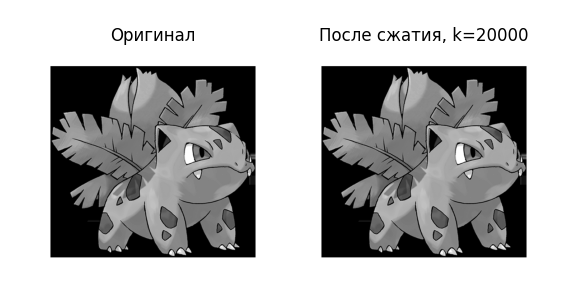
\includegraphics[width=0.85\linewidth]{graphics/k20000.png}} a) \\
\end{minipage}
\begin{minipage}[h]{1\linewidth}
\center{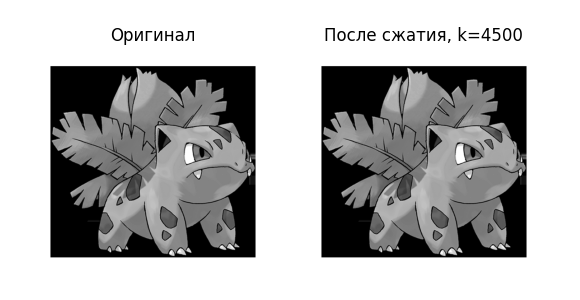
\includegraphics[width=0.85\linewidth]{graphics/k4500.png}} b) \\
\end{minipage}
\caption{Сжатие: a) k = 20000, b) k = 4500.}
\end{figure}

\begin{figure}[h]
\begin{minipage}[h]{1\linewidth}
\center{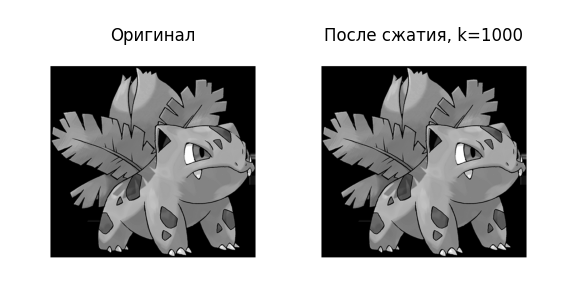
\includegraphics[width=0.85\linewidth]{graphics/k1000.png}} a) \\
\end{minipage}
\begin{minipage}[h]{1\linewidth}
\center{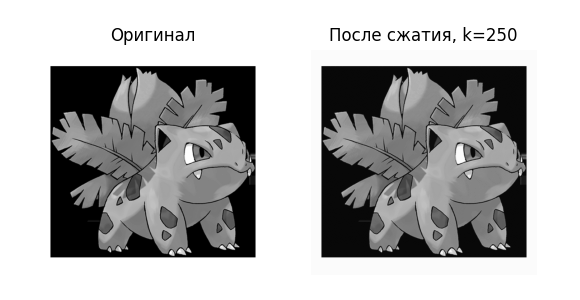
\includegraphics[width=0.85\linewidth]{graphics/k250.png}} b) \\
\end{minipage}
\caption{Сжатие: a) k = 1000, b) k = 250.}
\end{figure}

\begin{figure}[h]
\begin{minipage}[h]{1\linewidth}
\center{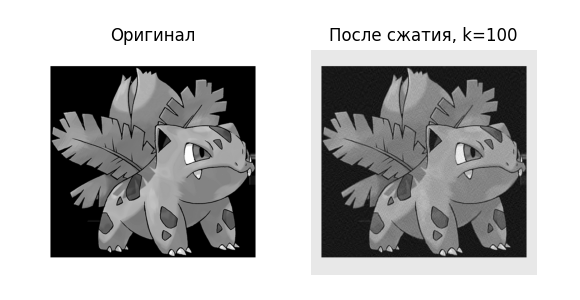
\includegraphics[width=0.85\linewidth]{graphics/k100.png}} a) \\
\end{minipage}
\begin{minipage}[h]{1\linewidth}
\center{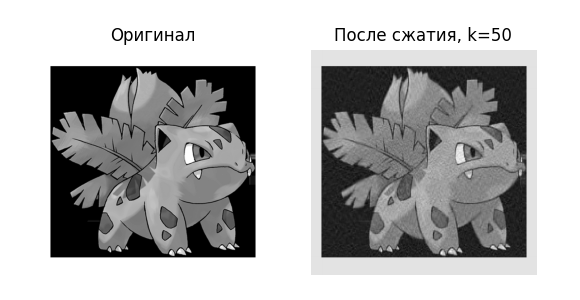
\includegraphics[width=0.85\linewidth]{graphics/k50.png}} b) \\
\end{minipage}
\caption{Сжатие: a) k = 100, b) k = 50.}
\end{figure}

\begin{figure}[h]
\begin{minipage}[h]{1\linewidth}
\center{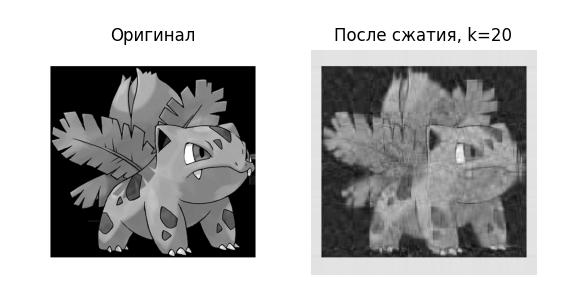
\includegraphics[width=0.85\linewidth]{graphics/k20.png}} a) \\
\end{minipage}
\begin{minipage}[h]{1\linewidth}
\center{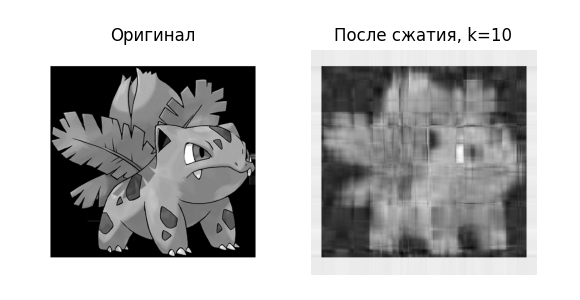
\includegraphics[width=0.85\linewidth]{graphics/k10.png}} b) \\
\end{minipage}
\caption{Сжатие: a) k = 20, b) k = 10.}
\end{figure}

\begin{figure}[h]
\begin{minipage}[h]{1\linewidth}
\center{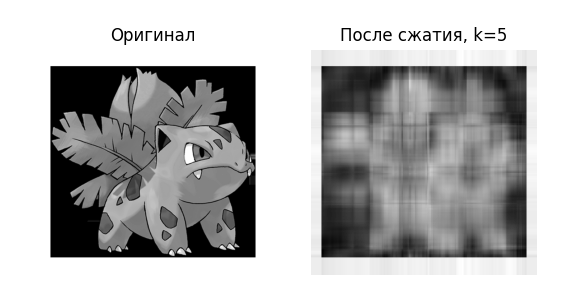
\includegraphics[width=0.85\linewidth]{graphics/k5.png}} a) \\
\end{minipage}
\begin{minipage}[h]{1\linewidth}
\center{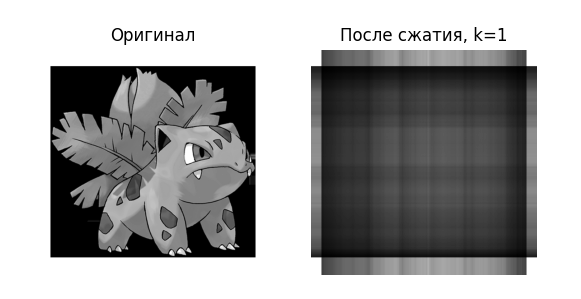
\includegraphics[width=0.85\linewidth]{graphics/k1.png}} b) \\
\end{minipage}
\caption{Сжатие: a) k = 5, b) k = 1.}
\end{figure}
\newpage
\,
\newpage
\,
\newpage
\,
\newpage
\,
\newpage
Заметно, что уже при $k \geq 5$ становится возможным различить черты Ивизавра, а при $k \geq 50$ сжатое изображение становится практически неотличимым от оригинала.\\
\\
Далее проанализируем, сколько памяти мы сэкономили, вычислим "вес" исходного изображения и сжатого. Результаты представлены в таблице 1.
\newpage
\begin{center}
Таблица 1 -- Сравнительные результаты работы программы\\

\begin{tabular}{ |c|c|c|c|c| } 
 \hline
k & Различим ли Ивизавр? & Вес оригинала  & Вес сжатого & \% сжатия \\
\hline
$2 \cdot 10^4$ & да, как оригинал & $451725$  & $451725$ & 0.00 \\
 \hline
$4500$ & да, как оригинал & $451725$ & $451725$ & 0.00  \\
 \hline
$10^3$ & да, как оригинал & $451725$ & $451725$ & 0.00  \\
 \hline
$250$ & да, как оригинал & $451725$ & $237750$ & 47.37 \\
 \hline
$100$ & да, как оригинал & $451725$ & $95100$ & 78.95 \\
 \hline
$50$ & да & $451725$ & $47550$ & 89.47 \\
 \hline
$20$ & да, отдаленно & $451725$ & $19020$ & 95.79 \\
 \hline
$10$ & да, отдаленно & $451725$ & $9510$ & 97.89 \\
 \hline
$5$ & нет & $451725$ & $4755$ & 98.95 \\
 \hline
$1$ & нет, совсем & $451725$ & $951$ &  99.79 \\
 \hline
\end{tabular}
\end{center}

\subsection{Анализ результатов и вывод}

Заметим, что при степени сжатия примерно на $90\%$ изображение все еще остается различимым . В частности, при $k \geq 5$ становится возможным различить черты Ивизавра, а при $k \geq 50$ сжатое изображение становится практически неотличимым от оригинала.\\
\\
  Таким образом, можно сделать вывод о том, что применение SVD-разложения является довольно эффективным инструментом сжатия изображений с минимальными потерями качества результата.

\end{document}













